\documentclass{standalone}
\usepackage{tikz}
\usepackage{tkz-euclide}
\usepackage{ctex}
\setCJKmainfont{Noto Serif CJK SC}
\usepackage{chemfig,siunitx}
\begin{document}
\small
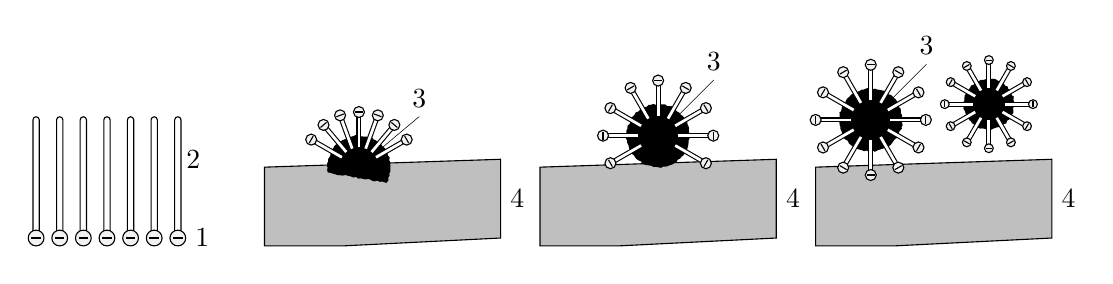
\begin{tikzpicture}[scale=1]
  \begin{scope}
    \foreach \x in {-0.9,-0.6,-0.3,0,0.3,0.6,0.9}
    {
      \draw(\x-0.04,0)--++(0,1.5)arc(180:0:0.04)--++(0,-1.5);
      \draw[fill=lightgray!20](\x,0)circle(0.1);
      \draw(\x-0.06,0)--(\x+0.06,0);
    }
    \node at (1,0)[right]{1};
    \node at (1,1)[inner sep=0pt,right]{2};
  \end{scope}
  \begin{scope}[xshift=2cm]
    \draw[fill=lightgray](0,-0.1)--(1,-0.1)--(3,0)--(3,1)node[midway,right]{4}--(0,0.9)--cycle;
    \begin{scope}[xshift=1.2cm,yshift=0.9cm]
      \fill[decorate,decoration={random steps,amplitude=0.1mm,segment length=0.3mm}](190:0.4)arc(190:-30:0.4)--cycle;
      \foreach \x in {30,50,70,90,110,130,150}
      {
        \draw[double distance=1pt](\x:0.25)--(\x:0.7);
        \draw[fill=lightgray!20](\x:0.7)circle(0.07);
        \draw(\x:0.7)--++(90+\x:0.05)(\x:0.7)--++(-90+\x:0.05);
      }
      \draw[very thin](0,0)--(40:1)node[above]{3};
    \end{scope}
  \end{scope}
  \begin{scope}[xshift=5.5cm]
    \draw[fill=lightgray](0,-0.1)--(1,-0.1)--(3,0)--(3,1)node[midway,right]{4}--(0,0.9)--cycle;
    \begin{scope}[xshift=1.5cm,yshift=1.3cm]
      \fill[decorate,decoration={random steps,amplitude=0.1mm,segment length=0.3mm}](0,0)circle(0.4);
      \foreach \x in {-30,0,...,210}
      {
        \draw[double distance=1pt](\x:0.25)--(\x:0.7);
        \draw[fill=lightgray!20](\x:0.7)circle(0.07);
        \draw(\x:0.7)--++(90+\x:0.05)(\x:0.7)--++(-90+\x:0.05);
      }
      \draw[very thin](0,0)--(45:1)node[above]{3};
    \end{scope}
  \end{scope}
  \begin{scope}[xshift=9cm]
    \draw[fill=lightgray](0,-0.1)--(1,-0.1)--(3,0)--(3,1)node[midway,right]{4}--(0,0.9)--cycle;
    \begin{scope}[xshift=0.7cm,yshift=1.5cm]
      \fill[decorate,decoration={random steps,amplitude=0.1mm,segment length=0.3mm}](0,0)circle(0.4);
      \foreach \x in {0,30,...,330}
      {
        \draw[double distance=1pt](\x:0.25)--(\x:0.7);
        \draw[fill=lightgray!20](\x:0.7)circle(0.07);
        \draw(\x:0.7)--++(90+\x:0.05)(\x:0.7)--++(-90+\x:0.05);
      }
      \draw[very thin](0,0)--(45:1)node[above]{3};
    \end{scope}
    \begin{scope}[xshift=2.2cm,yshift=1.7cm,scale=0.8]
      \fill[decorate,decoration={random steps,amplitude=0.1mm,segment length=0.3mm}](0,0)circle(0.4);
      \foreach \x in {0,30,...,330}
      {
        \draw[double distance=1pt](\x:0.25)--(\x:0.7);
        \draw[fill=lightgray!20](\x:0.7)circle(0.07);
        \draw(\x:0.7)--++(90+\x:0.05)(\x:0.7)--++(-90+\x:0.05);
      }
    \end{scope}
  \end{scope}
\end{tikzpicture}
\end{document}